\documentclass[tikz,border=15pt]{standalone}
\usepackage{amsmath,amssymb}
\usetikzlibrary{calc}

\begin{document}
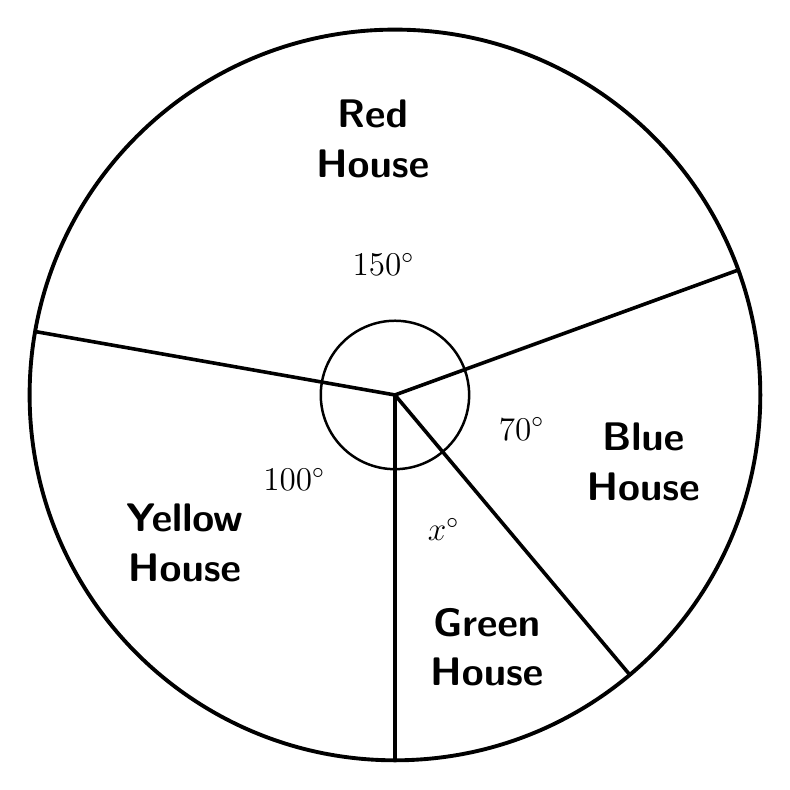
\begin{tikzpicture}[scale=1.45]
    \def\r{3.2} % radius of pie chart
    \def\rarc{0.65} % radius of central angle arcs
    
    % Circle boundary
    \draw[line width=1.4pt] (0, 0) circle (\r);
    
    % Sector angles:
    % Red House: 150 deg (20 to 170)
    % Yellow House: 100 deg (170 to 270)
    % Green House: 40 deg (270 to 310)
    % Blue House: 70 deg (310 to 380)
    
    % Radial dividing lines
    \draw[line width=1.3pt] (0, 0) -- (20:\r);
    \draw[line width=1.3pt] (0, 0) -- (170:\r);
    \draw[line width=1.3pt] (0, 0) -- (270:\r);
    \draw[line width=1.3pt] (0, 0) -- (310:\r);
    
    % Central angle arcs
    \draw[line width=0.9pt] (20:\rarc) arc (20:170:\rarc);
    \draw[line width=0.9pt] (170:\rarc) arc (170:270:\rarc);
    \draw[line width=0.9pt] (270:\rarc) arc (270:310:\rarc);
    \draw[line width=0.9pt] (310:\rarc) arc (310:380:\rarc);
    
    % Angle labels (positioned just outside central arcs)
    \node[font=\large\bfseries] at (95:1.15) {$150^\circ$};
    \node[font=\large\bfseries] at (220:1.15) {$100^\circ$};
    \node[font=\large\bfseries] at (290:1.25) {$x^\circ$};
    \node[font=\large\bfseries] at (345:1.15) {$70^\circ$};
    
    % Category labels in outer zone of sectors
    \node[font=\Large\sffamily\bfseries, align=center] at (95:2.25) {Red\\House};
    \node[font=\Large\sffamily\bfseries, align=center] at (215:2.25) {Yellow\\House};
    \node[font=\Large\sffamily\bfseries, align=center] at (290:2.35) {Green\\House};
    \node[font=\Large\sffamily\bfseries, align=center] at (345:2.25) {Blue\\House};
    
\end{tikzpicture}
\end{document}
